\documentclass[12pt]{article}
\usepackage[margin=1cm,left=2cm,includefoot]{geometry}
\usepackage{graphicx}
\usepackage{indentfirst} %indent fisrt line in section
\usepackage{subfig} %for mutiple figure strcutures
\usepackage[nottoc]{tocbibind}
\usepackage[numbers,sort&compress]{natbib} %for cite to give ranges
\usepackage[onehalfspacing]{setspace} %1.5 linespacing (according to stackexchange - not really 1.5...)


\begin{document}

\begin{titlepage}
	\begin{center}
		\begin{figure}[h]
		\centering
		
\includegraphics[scale=1]{img/asd}
		\end{figure}	
	\vspace{2cm}
	\huge{\bfseries Brain lesion detection using neural networks}\\
	\vspace{2cm}
	\large{Neural networks course project}\\
	\vspace{5cm}
	\end{center}
	\begin{flushright}
	\large Done by: EKSfmu-16 gr. st. Arūnas Butkus
	\linebreak
	\large Checked by: prof. dr. Artūras Serackis
	\end{flushright}
	\vspace{6cm}
	\begin{center}
	\textsc{Vilnius, 2017}
	\end{center}
\end{titlepage}


\section{Introduction}
\label{sec:intro}

Magnetic resonance imaging (MRI) scans allows seeing the situation within the body. It is primary means of seeing if there are any issues with the brain. The scan in itself does not tell if there is an issue and a trained medic needs to determine if there is an issue. One of such issues is the blood spill in the brain – lesion for short. There are cases where lesions are small and hard to notice and require an expert to spot them; sometimes they are a huge glob.

So the goal here is to see if it is possible to implement neural networks to at least classify if there is an issue, and ideally mark the lesion area. And here I look through some MATLAB solutions to at least similar problems proposed by others, looking for a method that might work to some degree.

\section{Potential MATLAB algorithms}
\label{sec:poMaAl}

\subsection{Image Segmentation tutorial}
\label{ssec:imSegTut}

Started off by looking what's available online as far as implementation in MALTAB is concerned. Specifically for lesion delineation there is few options, and fewer that implement neural networks. The ones I look at don't really use neural networks I guess, but whatever. 

So first off was image segmentation tutorial \cite{matlabSegmentationTutorial}. And really that is what I went most in depth with. This shows region growing methods to find nickels and dimes in the image. 

\begin{figure}[!htb]
\centering
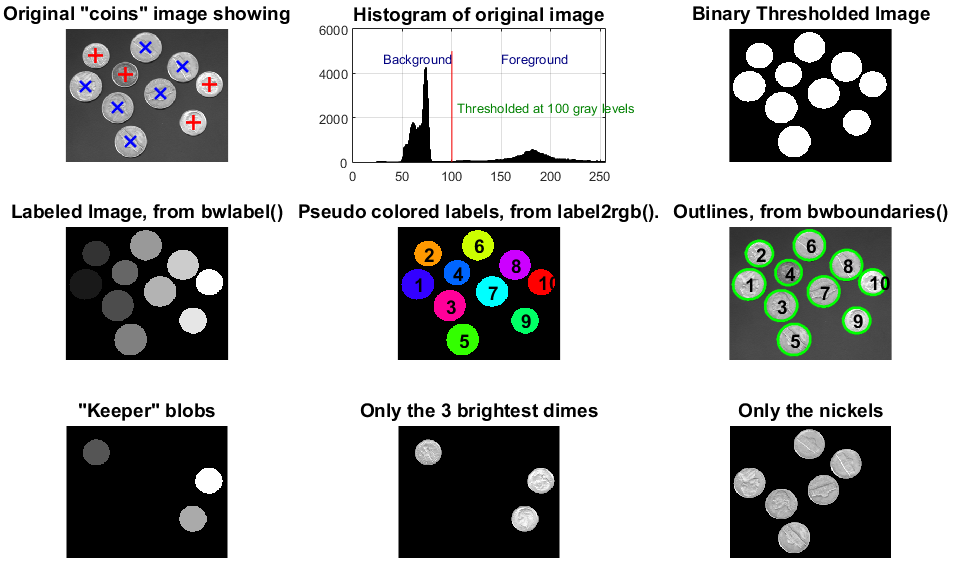
\includegraphics[width=0.8\textwidth]{img/coinsThresholdedSegmentation}
\caption{Results shown by the algorithm}
\label{fig:coinsThresholdedSegmentation}
\end{figure}

It starts off by finding minima in the image. These points are grown using binary images. These are obtained by thresholding since in the grayscale image histogram clearly seen that some objects have clearly higher luminosity than others. In this case the coins have higher luminosity than the wooden background.

Once the regions are obtained they then are classified using overall blob area – whether area is larger or smaller than a pre-picked value. This part could be made with a neural network instead. Though in either case algorithms would fail if other image provided would be from a different distance and neither the hardcoded size thresholds, neither trained neural network wouldn't be able to say with certainty whether this is nickel or dime. So this points out that area alone is not sufficient feature for neural network even in this simple case.

\subsection{Tumor detectors}
\label{ssec:tumors}

Of the ones that worked there’s two - Automatic segmentation of brain tumor in MR images\cite{matlabTumor} and, seemingly a rip-off from aforementioned, Brain tumor detection from MRI images using anisotropic filter and segmentation image processing\cite{matlabTumor2}. As for why I called it a rip-off, second one is two years later and uses identical customer helper function, but, again, whatever.

\begin{figure}[!htb]
\centering
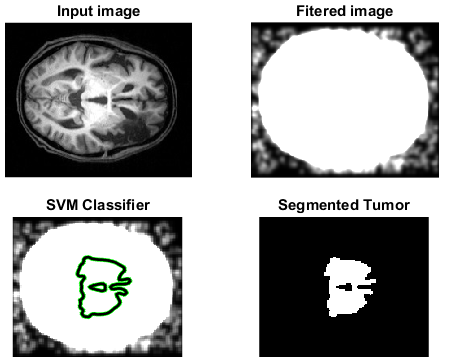
\includegraphics[width=0.8\textwidth]{img/tumor2}
\caption{Older tumor detection algorithm\cite{matlabTumor} results for lesion detection.}
\label{fig:tumor1}
\end{figure}

\begin{figure}[!htb]
\centering
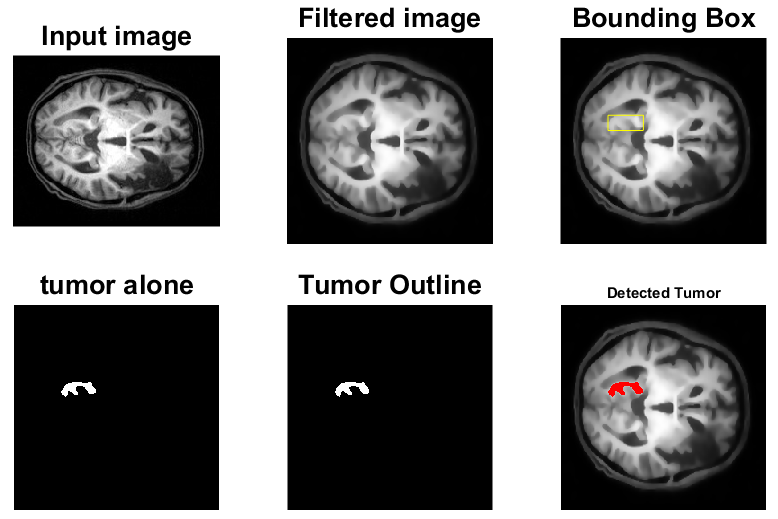
\includegraphics[width=0.8\textwidth]{img/tumerFull}
\caption{Newer tumor detection algorithm\cite{matlabTumor2} results for lesion detection.}
\label{fig:tumor2}
\end{figure}

In theory these try to find tumors in the brain so I guess it is no surprise that neither first one (Fig.~\ref{fig:tumor1}) nether the second one (Fig.~\ref{fig:tumor2}) is able to find lesion area. So I moved on.

\section{Feature extraction for neural network}
\label{sec:featnn}

This is where I spent most of my time. Created 4 functions that would be useful if I will get stupid enough to ever go back to this approach. First one is \texttt{NNCP\_Image\_Segmentation\_edgetech.m} – customized version of Image Segmentation Tutorial mentioned before. And in the end creates three structures that I intended to use as inputs when training neural network. These structures contain largest area blob definition as given by MATLAB function \texttt{regionprops}. That gives a lot of numbers (Fig.~\ref{fig:matalbNumbers}) which is good when going for precision in neural networks, not so much when thinking of training speed. 

\begin{figure}[!htb]
\centering
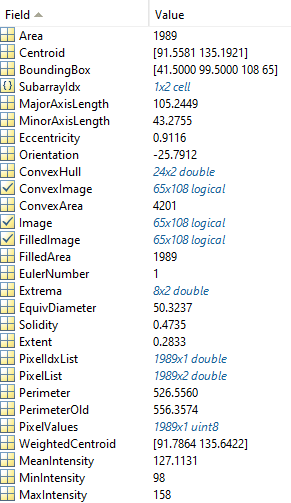
\includegraphics[width=0.3\textwidth]{img/MATLAB_2017-12-17_15-38-27}
\caption{My feature extraction/segmentation results.}
\label{fig:matalbNumbers}
\end{figure}

As to why three structures it's because I threshold binary image at three different normalized levels~-~0.3, 0.4 and 0.6~-~just some random numbers. Did not give much thought to these, just eyeballed them since in the end brain grayscale image is not nearly as clear cut as with coins on a table. So these threshold give varying blobs in cases which is good enough. In this case I'm thinking of one case in particular that I noticed while testing out: at one threshold level this large lesioned area is within the blob; at another level it is entirely outside; so I figure neural network would see this sudden disappearance of large blob area and would think that that is due to lesion.

\begin{figure}[!htb]
\centering
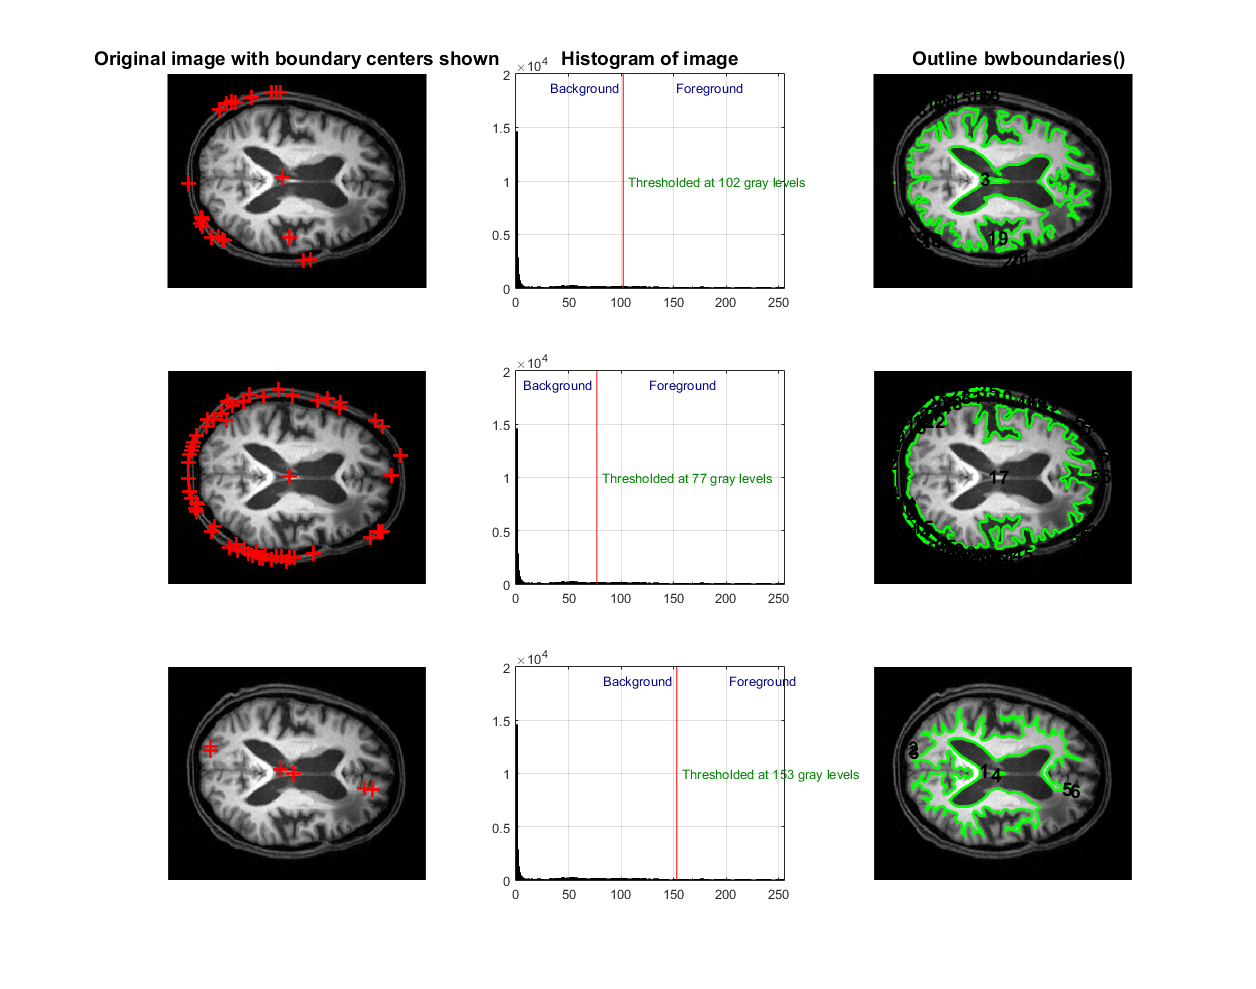
\includegraphics[width=0.8\textwidth]{img/meh}
\caption{My feature extraction/segmentation results.}
\label{fig:meh}
\end{figure}

Anyway, I made the script be able to optionally draw some graphs (Fig.~\ref{fig:meh}). These show blob centers on the left column, image histogram with threshold level depicted in the middle column, blob boundaries and numbers in the right column. In this case I show off the idea I had about the thresholds making blob encompass the lesion or not.

Other functions are variable/data processing shifting around and overall repetition speed up and automatization. Like the second one: \texttt{NNCP\_ImageCycling.m}. This one in essence takes a .nii file, which is 3D, and makes a bunch of 2D slices saving those as separate images (thanks to \texttt{nifti2slices.m}. Then it goes through each of those slices and sends them off to \texttt{NNCP\_Image\_Segmentation\_edgetech.m} to extract features. It concatenates those features for all slices it made and sends them on to whoever called this function. There's other bells and whistles that ease the life but, once more, whatever.

Third function, which time wise came to be first of these four, is: \texttt{nifti2slices.m}. Returns image data of specified slice or slices back to the function that requested it. Lots of fun with automation, but, effectively, ineffective use of time.

And lastly the intended front-end function: \texttt{NNCP\_ET\_NN.m}. This is what initiates feature gathering from, at this point, 6 .nii files and then parses them into a double type values matrix, since that is what I though neural network trainers would want. Also it generates the goals vector, currently gave it values by visual inspection, but I might add script for getting values from the lesion .nii files that I have.

\begin{figure}[!htb]
\centering
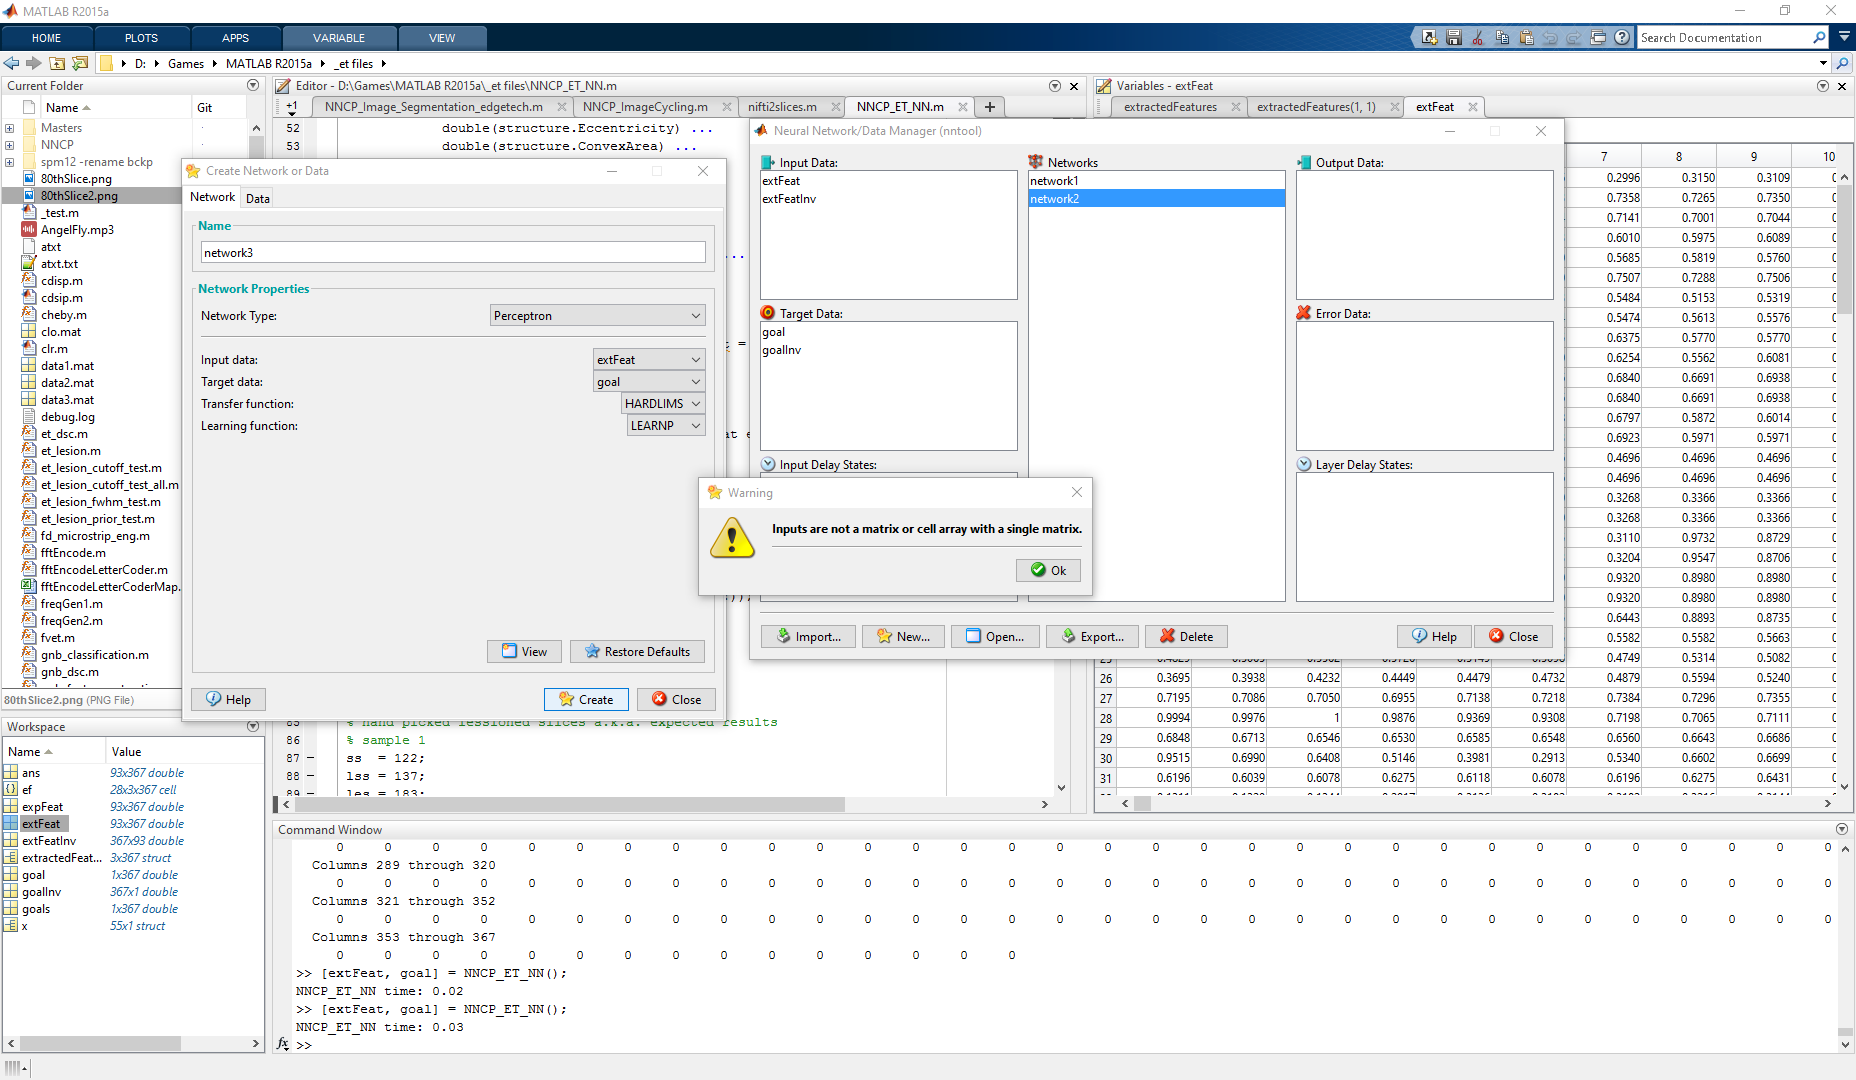
\includegraphics[width=0.8\textwidth]{img/MATLAB_2017-12-17_13-42-07}
\caption{How far I've got.}
\label{fig:fuckItImOut}
\end{figure}

And at this point I hit \texttt{nntool}. At best getting error that it does not like my inputs matrix (Fig.~\ref{fig:fuckItImOut}). I formatted data, input and output, like for apples and pears from way back when. Here functions didn't like that and I don't have motivation, energy, drive or whatever to bash my head against it till something eventually works.

\section{Conclusions}
\label{sec:conclusions}

So this is not even like the embedded systems laboratory works, where in conclusion I just said "It works". Here nothing works and I do not have in me whatever is needed to make it work. Working on images of neural networks with neural networks destroys too many neural networks by way of stress and at times anger so, for final time, whatever.

Here is the thing – neural networks are a difficult construct, especially so when trying to find a region within an image. Even more so when said image is grayscale and asymmetric and the region to look for may be there, may not be, may be nigh a circle, may be a small noodle on the side. What I am getting at is that in my situation neural networks are way too difficult a concept for me to implement in a way that would yield some conclusive results. I admit being at fault here since I left myself two days here instead of working intermittently over all semester, but eitherway from what i understand i didn't have enough data to train proper image recognition neural network. And utilizing some great MATLAB toolboxes, like SPM12, gives better results with less hassle; also allows 3-dimensional work instead of 2D (referring to J.C. Griffis idea \cite{griffis2016voxel}).


\clearpage

\clearpage
\nocite{*}
\bibliographystyle{unsrt}
\bibliography{References}


\end{document}